\documentclass[12pt]{ucsddissertation}
% mathptmx is a Times Roman look-alike (don't use the times package)
% It isn't clear if Times is required. The OGS manual lists several
% "standard fonts" but never says they need to be used.
\usepackage{mathptmx}
\usepackage[NoDate]{currvita}
\usepackage{array}
\usepackage{tabularx}
\usepackage{booktabs}
\usepackage{ragged2e}
\usepackage{microtype}
\usepackage[breaklinks=true,pdfborder={0 0 0}]{hyperref}
\usepackage{graphicx}
\usepackage{subcaption}
\usepackage{amsmath}
\usepackage{enumitem}
\usepackage{arydshln}
\AtBeginDocument{%
	\settowidth\cvlabelwidth{\cvlabelfont 0000--0000}%
}

%commands

\newcommand{\sword}{SwordBox}
\newcommand{\thesistitle}{Enze Liu's Thesis Title \\ Blah blah}

\usepackage{multirow}
\usepackage{tikz}
\newcommand*\nullcirc[1][1ex]{\tikz\draw (0,0) circle (3pt);} 
\newcommand*\halfcirc[1][1ex]{%
  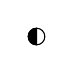
\begin{tikzpicture}
  \draw[fill] (0,0)-- (90:3pt) arc (90:270:3pt) -- cycle ;
  \draw (0,0) circle (3pt);
  \end{tikzpicture}}
\newcommand*\fullcirc[1][1ex]{\tikz\fill (0,0) circle (3pt);} 

% OGS recommends increasing the margins slightly.
\increasemargins{.1in}

% These are just for testing/examples, delete them
\usepackage{trace}
%\usepackage{showframe} % This package was just to see page margins
\usepackage[english]{babel}
\usepackage{blindtext}
\usepackage{ifthen}
\usepackage[normalem]{ulem} % for \sout
\usepackage{xcolor}
\usepackage{amssymb}

\newcommand{\ra}{$\rightarrow$}
\newboolean{showedits}
\setboolean{showedits}{true} % toggle to show or hide edits
\ifthenelse{\boolean{showedits}}
{
	\newcommand{\ugh}[1]{\textcolor{red}{\uwave{#1}}} % please rephrase
	\newcommand{\ins}[1]{\textcolor{blue}{\uline{#1}}} % please insert
	\newcommand{\del}[1]{\textcolor{red}{\sout{#1}}} % please delete
	\newcommand{\chg}[2]{\textcolor{red}{\sout{#1}}{\ra}\textcolor{blue}{\uline{#2}}} % please change
}{
	\newcommand{\ugh}[1]{#1} % please rephrase
	\newcommand{\ins}[1]{#1} % please insert
	\newcommand{\del}[1]{} % please delete
	\newcommand{\chg}[2]{#2}
}

\newboolean{showcomments}
\setboolean{showcomments}{true}
% \setboolean{showcomments}{false}
\newcommand{\id}[1]{$-$Id: scgPaper.tex 32478 2010-04-29 09:11:32Z oscar $-$}
\newcommand{\yellowbox}[1]{\fcolorbox{gray}{yellow}{\bfseries\sffamily\scriptsize#1}}
\newcommand{\triangles}[1]{{\sf\small$\blacktriangleright$\textit{#1}$\blacktriangleleft$}}
\ifthenelse{\boolean{showcomments}}
%{\newcommand{\nb}[2]{{\yellowbox{#1}\triangles{#2}}}
{\newcommand{\nbc}[3]{
 {\colorbox{#3}{\bfseries\sffamily\scriptsize\textcolor{white}{#1}}}
 {\textcolor{#3}{\sf\small$\blacktriangleright$\textit{#2}$\blacktriangleleft$}}}
 \newcommand{\version}{\emph{\scriptsize\id}}}
{\newcommand{\nbc}[3]{}
 \renewcommand{\ugh}[1]{#1} % please rephrase
 \renewcommand{\ins}[1]{#1} % please insert
 \renewcommand{\del}[1]{} % please delete
 \renewcommand{\chg}[2]{#2} % please change
 \newcommand{\version}{}}
\newcommand{\nb}[2]{\nbc{#1}{#2}{orange}}

\definecolor{ibcolor}{rgb}{0.4,0.6,0.2}
\newcommand\iv[1]{\nbc{IB}{#1}{ibcolor}}
\usepackage{wasysym}
\newcommand\yesml[1]{\nbc{ML {\textcolor{yellow}\sun}}{#1}{mircolor}}

\definecolor{sgcolor}{rgb}{0.2,0.0,0.5}
\newcommand\sg[1]{\nbc{SG}{#1}{sgcolor}}

\definecolor{samcolor}{rgb}{0.2,0.4,0.2}
\newcommand\sam[1]{\nbc{SC}{#1}{samcolor}}

\definecolor{hccolor}{rgb}{0.21,0.54,0.84}
\newcommand\hc[1]{\nbc{HC}{#1}{hccolor}}

\definecolor{ideacolor}{rgb}{1.0,0,0.5}
\newcommand\idea[1]{\nbc{IDEA}{#1}{ideacolor}}


\definecolor{abstractcolor}{rgb}{0.0,0.5,1.0}
\newcommand\rabstract[1]{\nbc{ABSTRACT}{#1}{abstractcolor}}

\definecolor{introcolor}{rgb}{0.0,1.0,0.5}
\newcommand\rintro[1]{\nbc{INTRO}{#1}{introcolor}}

\definecolor{papercolor}{rgb}{1.0,1.0,0.0}
\newcommand\rpaper[1]{\nbc{PAPER}{#1}{papercolor}}

\definecolor{multicolor}{rgb}{1.0,0,0}
\newcommand\rmulti[1]{\nbc{MULTI}{#1}{multicolor}}

% Todo Command
\definecolor{todocolor}{rgb}{0.9,0.1,0.1}
\newcommand{\todo}[1]{\nbc{TODO}{#1}{todocolor}}


\overfullrule5pt
% ---

% Required information
\title{\thesistitle}
\author{Enze Liu}
\degree{Computer Science}{Doctor of Philosopy}
% Each member of the committee should be listed as Professor Foo Bar.
% If Professor is not the correct title for one, then titles should be
% omitted entirely.
\cochair{Professor Stefan Savage}
\cochair{Professor Geoffrey M. Voelker}
% Your committee members (other than the chairs) must be in alphabetical order
\committee{Professor KC Claffy}
\committee{Doctor David D Clark}
\committee{Professor Terrance August}
\degreeyear{2025}

% Start the document
\begin{document}
% Begin with frontmatter and so forth
\frontmatter
\maketitle
\makecopyright
\makesignature
% Optional
\begin{dedication}
\setsinglespacing
\raggedright % It would be better to use \RaggedRight from ragged2e
\parindent0pt\parskip\baselineskip

\textit{To Mom and Dad, who raised me as a human being; to Stefan and Geoff, who raised me as a researcher; and to everyone who believed in and invested in me --- you made me who I am today.}


% In recognition of reading this manual before beginning to format the
% doctoral dissertation or master's thesis; for following the
% instructions written herein; for consulting with OGS Academic Affairs
% Advisers; and for not relying on other completed manuscripts, this
% manual is dedicated to all graduate students about to complete the
% doctoral dissertation or master's thesis.

% In recognition that this is my one chance to use whichever
% justification, spacing, writing style, text size, and/or textfont that
% I want to while still keeping my headings and margins consistent.
\end{dedication}
% Optional
\begin{epigraph}
\vskip0pt plus.5fil
\setsinglespacing
\begin{flushright}
``It takes a village to raise a child.''\\
\vskip\baselineskip
% -Voltaire \textit{Candide}\par
-African Proverb
\end{flushright}

\vfil
\begin{center}

% \noindent “It must be considered that there is nothing more difficult to carry out, nor more
% doubtful of success, nor more dangerous to handle, than to initiate a new order of things.”

\vskip\baselineskip
% \hskip0pt plus1fil -Niccolo Machiavelli \textit{The Prince}\hskip0pt plus4fil\null

\end{center}
\vfil
``My ears had heard of you but now my eyes have seen you.''\\

\vskip\baselineskip
-Job 42:5, \textit{NIV}

\vfil
\end{epigraph}

% Next comes the table of contents, list of figures, list of tables,
% etc. If you have code listings, you can use \listoflistings (or
% \lstlistoflistings) to have it be produced here as well. Same with
% \listofalgorithms.
\tableofcontents
\listoffigures
\listoftables

% Preface
% \begin{preface}
% \todo{Write a preface - take a look at some examples because it seems rather free form}
% Almost nothing is said in the manual about the preface. There is no
% indication about how it is to be typeset. Given that, one is forced to
% simply typeset it and hope it is accepted. It is, however, optional
% and may be omitted.
% \end{preface}

% Your fancy acks here. Keep in mind you need to ack each paper you
% use. See the examples here. In addition, each chapter ack needs to
% be repeated at the end of the relevant chapter.
\begin{acknowledgements}

% Chapter~\ref{chap:swordbox} is a partial reprint of work submitted to multiple USENIX and ACM
% conferences under the title "SwordBox: Accelerating Shared Access in RDMA-based Disaggregated
% Memory. Stewart Grant, Alex C. Snoeren. This dissertations author was the primary investigator and
% author of this paper.
% %%
% Chapter~\ref{chap:rcuckoo} is a partial reprint of work submitted to multiple USENIX conferences
% under the title "Cuckoo for Clients: Disaggregated Cuckoo Hashing. Stewart Grant, Alex C. Snoeren.
% This dissertations author was the primary investigator and author of this paper.

I would like to acknowledge some people here.

% This dissertation has been extraordinarily influenced by Anil Yelam, my closest collaborator. Thank you
% for all the time you spent working on our collaborations, and the hours spent discussing and
% debating system designs and performance results. I'm forever grateful. To Maxwell Bland, your
% research energy is unmatched and without your help we would never have have acquired any SmartNICs.
% And Alex (Enze) Liu for his superior knowledge of Python and unmatched focus on research.  Thank you
% to all of the members of the Systems and Networking group at UCSD, especially the optical networking
% group for your feedback and guidance during the first years of my PhD.

% Thank you to Meta for funding my research and providing me with the opportunity to work on resource
% disaggregation, Cavium for the generous donation of two SmartNICs, and to ARPAe for funding my first
% years of research.

% I'd like to thank all of the members of 3140 for their collaboration and friendship over the years.
% It's truly the best office, Chez bob volunteers for keeping me fed, and to my friends for the
% support. Camille Rubel thanks for having the best climbing schedule in the world, Phillip Arndt for
% pushing my limits, and Camille Moore for keeping me on my toes.
\todo{double check I thanked everyone}


\end{acknowledgements}

% Stupid vita goes next
\begin{vita}
\noindent
\begin{cv}{}
\begin{cvlist}{}
\item[2012-2016] Bachelor of Science, Software Engineering, Beijing Institute of Technology
\item[2016-2018] Master of Science, Computer Science, University of Chicago
\item[2019-2025] Doctor of Philosophy, Computer Science, University of California San Diego
\end{cvlist}
\end{cv}

% This puts in the PUBLICATIONS header. Note that it appears inside
% the vita environment. It is optional.
\publications

\noindent Deepak Bansal, Gerald DeGrace, Rishabh Tewari, Michal Zygmunt, and James Grantham, Silvano
Gai, Mario Baldi, Krishna Doddapaneni, Arun Selvarajan, Arunkumar Arumugam, Balakrishnan Raman,
Avijit Gupta, Sachin Jain, Deven Jagasia, Evan Langlais, Pranjal Srivastava, Rishiraj Hazarika,
Neeraj Motwani, Soumya Tiwari, Stewart Grant, Ranveer Chandra, and Srikanth Kandula . 2023.
Disaggregating Stateful Network Functions. In proceedings of 20th USENIX Symposium on Networked
Systems Design and Implementation (NSDI '23).  Usenix Association, Boston MA, USA, April 2018, 1469--1487. \\

\noindent Stewart Grant, Anil Yelam, Maxwell Bland, and Alex C. Snoeren. 2020. SmartNIC Performance
Isolation with FairNIC: Programmable Networking for the Cloud. In Proceedings of the Annual
conference of the ACM Special Interest Group on Data Communication on the applications,
technologies, architectures, and protocols for computer communication (SIGCOMM '20). Association for
Computing Machinery, Virtual Event, August 2020, 681–693.\\

\noindent Stewart Grant, Hendrik Cech, and Ivan Beschastnikh. 2018. Inferring and asserting
distributed system invariants. In Proceedings of the 40th International Conference on Software
Engineering (ICSE '18). Association for Computing Machinery, Gothenberg, Sweden, July 2018, 1149–1159.\\


% This puts in the FIELDS OF STUDY. Also inside vita and also
% optional.
% \fieldsofstudy
% \noindent Major Field: Computer Science
\end{vita}

% Put your maximum 350 word abstract here.
\begin{dissertationabstract} 
%%	
Resource disaggregation proposes a next-generation architecture for data center resources. System
components like compute, memory, storage, and accelerators are separated from one another by a fast
network and composed dynamically into virtual servers when required. This paradigm promises to
dramatically improved resource utilization, scalability, and flexibility, but introduces substantial
challenges in terms of performance and fault tolerance. Memory is among the most difficult resources
to disaggregate. CPUs currently expect DRAM to have ultra low latency, high bandwidth, and to share it's
failure domain. In particular increased latency from network round trips dramatically shifts the
performance of existing shared data structures designed for local DRAM.

In this dissertation I demonstrate the challenges of sharing disaggregated memory and show that
programmable network devices can be used to significantly improved system performance. I present two
systems: First {\sword} which utilizes a centralized programmable switch to cache data structure
state and dramatically improve key-value workload performance. Second I present a new key-value
store RCuckoo which is designed to leverage RDMA and reduce round trips when accessed by CPUs over a
network. Both systems demonstrate significant performance improvements over the existing state of
the art.

\end{dissertationabstract}

% This is where the main body of your dissertation goes!
\mainmatter

% Optional Introduction
\begin{dissertationintroduction}


\textit{What should a data center server look like?} Twenty years ago, a data center operator may
have argued for the simplicity of homogeneity over optimal performance, reasoning that carefully
picked commodity hardware at a given price point would yield the best cost-performance tradeoffs and that the
performance gains of next-generation hardware would quickly erase any benefits made by specializing
servers due to Dennard scaling~\cite{moore}.

Since then, both Moore's law and Dennard scaling have slowed down dramatically. CPU clock speeds and
memory density improvements have stagnated, leaving operators to fight tooth and claw to enjoy the
efficiency gains of prior decades. The effect is that new technologies are being introduced to
achieve scaling. CPUs are now monstrously parallel. Custom accelerators are common for specialized
workloads like video coding and machine learning. Indeed, the modern data center is a hodgepodge of
heterogeneous hardware (GPUs, TPUs, DPUs, SmartNICs, and
FPGAs)~\cite{dsnf,azure-smartnic,tpu,nitro}, and various new memory offerings and tiers like
NVMe~\cite{decible}. Today, the number of server types in a data center, conservatively, is in the
dozens. At the time of writing, EC2 has 84 listed instance types~\cite{ec2-offer} for their
customers to design their services. The trend is clear: in search of efficiency, data center and
server design is increasingly heterogeneous, with servers being designed for specific applications
and workloads.

Resource disaggregation is a new architectural paradigm for data center resources aimed at improving
efficiency and managing increased heterogeneity. In the disaggregated model, a server's resources do
not monolithically reside in a 1U, 2U, or 4U server form factor. Instead, each resource (i.e.,
compute, memory, storage) is deployed separately to a dedicated machine and interconnected via a
fast network. Servers are composed dynamically from these resources, which enables them to be
provisioned for their exact purpose~\cite{disandapp,infiniswap,blade-server,decible,legoos}. This
model enables resource pooling and sharing, which in turn leads to higher
efficiency~\cite{regions,fastswap,dsnf,aifm,supernic,ditto}.


% DRAM in particular has quickly become a precious resource in the data center. Main memory capacity,
% while growing has not kept up with CPU core counts. The result is that per-core memory capacity is
% less than 10 years ago~\cite{micron-memorywall}. New memory tiers like NVMe have been introduced to
% help alleviate memory pressure from applications, but the composition of these memory tiers, and the
% software to manage them are still undecided.

DRAM, in particular, has become a precious resource in data centers and is a focused target for
resource pooling~\cite{micron-memorywall}. The benefits of pooling are clear when examining a simple
bin packing problem. Consider two servers, each provisioned with 4GB of DRAM, and three jobs, each
requiring 2.5GB of memory. In a monolithic design, a scheduler can only place one job per machine or
risk swapping to disk. In a disaggregated model, the 4GB of memory could be placed in an 8GB pool,
which could be easily subdivided into three 2.5GB partitions. In the monolithic case, the unused
memory is stranded, while pooling reclaims stranded memory. More concretely, at data center levels,
practitioners have to provision their servers for the sum of peak demand; when resources are pooled,
they can be provisioned for the peak of the sum of demand, which can be significantly
lower~\cite{ dsnf, supernic}.

Disaggregation, in general, is only possible because of new fast networks. Commodity NICs now offer
400Gbps with expectations for continued growth to 800Gbps and above~\cite{cx8}. Network and memory
bandwidths are quickly approaching the same order of magnitude. At the same time, network stacks are
becoming lighter-weight through kernel bypass and CPU bypass technologies like DPDK~\cite{dpdk} and
RDMA~\cite{infiniband-spec}, enabling applications to more easily take advantage of the additional
bandwidth. Network devices themselves are becoming increasingly programmable, with multiple vendors
offering programmable SmartNICs, DPUs, and switches~\cite{tofino2,bluefield,pensando}. These two
trends have led to intra-rack latencies of 1-2{$\mu$}s, with the ability to inspect, cache, and
modify packets in flight at line rate.


Despite fast networks, memory disaggregation has remained elusive while storage, such as spinning
disks and solid-state drives, has seen widespread disaggregation. The reason for this contrast is
that storage device access latency is far higher than a network round trip. In the case of memory,
the opposite is true. Memory access latency is approximately 20 times lower than a network round
trip (50-100ns), effectively making it a separate tier of memory when placed across a network. While
there is ongoing research demonstrating the advantages of tracking cache lines over pages for remote
memory~\cite{kona}, the cost of fully disaggregating all memory is deemed too high~\cite{legoos}. A common
proposal for disaggregated memory is to have CPUs with a reasonably sized cache (e.g., 4GB) of DRAM
attached to them, along with software to manage and reduce the cost of remote
accesses~\cite{legoos}.

A large body of literature exists on disaggregated memory systems with a significant local cache.
Many of these systems intervene in the virtual memory system to decrease the cost of accessing
remote memory by employing prefetching and eviction strategies aimed at minimizing blocking remote
accesses~\cite{infiniswap,fastswap,leap,hydra}. Similarly, object-based disaggregated systems
utilize remotable objects with per-object tracking to mitigate the frequency of remote
accesses~\cite{aifm,carbink}. Additionally, compiler-based systems leverage static and dynamic
analysis to identify large, small, and hot objects for cache optimization~\cite{mira,trackfm}. These
systems primarily focus on analyzing memory access patterns and reducing the number of remote
accesses with decreasing volumes of local cache. However, they often overlook a critical aspect of
memory access: sharing. When memory is shared, access patterns alone are insufficient to minimize
round trips. Some degree of coherence must be maintained between remote caches, which is the primary
focus of this dissertation.


% %%
% Sharing data between multiple remote machines, where coherence between remote cores is required,
% leads to abysmal performance degradation (300x tail latencies in some cases)
% (Chapter~\ref{chap:swordbox}). Further complicating the design of shared data structures is that
% memory, once in a single fault domain, can fail, ripping a hole directly into a process's address
% space~\cite{amanda-hotnets,hydra,legoos}.

%%you have to add in a paragraph on current successful disaggregated systems

At its core, the challenge of sharing in disaggregated memory is serialization. When a data
structure is shared by multiple accessors, some mechanism must ensure the consistency of the data
structure. In a monolithic system, this is often achieved with locks or atomic operations. Across
machines, serialization is typically accomplished by either a centralized sequencer or a distributed
protocol. As a point of comparison, consider the differences between serialization in a traditional
RPC system and disaggregated memory. In an RPC system, requests arrive on a NIC and are delivered to
one or more CPU cores for processing~\cite{cuckoo-improvements,pilaf,herd,memc3,memcached}. If all
requests are routed through a single CPU core, it implicitly serializes operations by enqueueing the
RPC requests and servicing them one at a time. If the RPC service has multiple cores, any shared
structure can be protected via a lock or other synchronization mechanism in the RPC server's local
memory. In contrast, in a disaggregated system, no such server-side CPU exists. Or, if one does, it
is assumed to be low power and incapable of handling significant traffic. In the absence of such a
CPU, clients must enforce serialization amongst themselves.

In the absence of a serialization mechanism close to memory, clients must rely on the only mechanism
available in commodity systems: RDMA atomics. Throughout this dissertation, RDMA atomics will be
used as the backbone of all shared disaggregated data structures. They take the form of two
operations: compare-and-swap (CAS) and fetch-and-add (FAA), which execute with the same semantics as
their local counterparts but on the memory of a remote machine. While their semantics remain the
same, their performance is dramatically different. As noted before, the cost of executing a remote
operation is 20 times that of local memory. This latency inflates the size of critical sections
built with remote locks and leads to stale caches and poor performance for optimistic data
structures under contention~\cite{clover,sherman,fusee,race,rolex}.

\begin{center}
\textit{Data structures can be optimized for disaggregated memory by leveraging network programmability.} \\
\end{center}

This thesis statement is the core of the work presented in this dissertation. The challenges listed
above, while fundamental to the problem domain can be practically alleviated in a variety of ways by
exploiting modern network hardware. We provide evidence for the thesis statement above by addressing
the following two questions.
%%
\textit{Where and how should serialization occur?} The default answer to these questions is "on the
NIC" and "with RDMA atomic verbs." However, given the landscape of programmable in-network hardware,
our options are flexible. At rack-scale, both TORs and NICs offer serialization points. The
interface and mechanism for serialization can be customized using programmable hardware. For
instance, a switch could be programmed to maintain locks~\cite{netlock}, provide
sequencing~\cite{when-computer}, or directly implement contended functions~\cite{mind}.
Simultaneously, NICs, though lower bandwidth and less centralized than TORs, have the potential to
offer extended RDMA interfaces~\cite{prism} and implement OS functionality for remote
clients~\cite{clio, supernic}.
%%
\textit{What data structures should be used?} Few data structures are currently designed for remote
memory~\cite{clover,fusee,race,sherman,rolex,ditto}. While these systems resemble
RDMA~\cite{pilaf,herd,cell} and NUMA~\cite{flat-combining,hopscotch,bbn} systems of the past,
disaggregation requires special consideration for the network hardware it runs on. How can round
trips and access latencies be reduced? What data structures are easy to build, and which are hard?
These questions are a key focus of this dissertation.

This dissertation explores the design of shared data structures in disaggregated memory systems. I
introduce two systems, {\sword} and RCuckoo, which address the challenges of sharing and contending
access to remote memory. {\sword} (Chapter~\ref{chap:swordbox}) adopts a middlebox approach to
alleviate contention in shared data structures. Its key insight leverages the serialized view of
traffic at rack-scale TORs, caching data structure state on a programmable switch. Additionally, I
present RCuckoo (Chapter~\ref{chap:rcuckoo}), a fully disaggregated key-value store specifically
designed to enhance key-value locality. RCuckoo utilizes locality-sensitive hashing to improve
performance in reads, writes, locking, and fault recovery by minimizing round trips. {\sword}
demonstrates significant improvements in both throughput (up to 30x) and tail latency (up to 300x),
while RCuckoo meets or surpasses the performance of all state-of-the-art disaggregated key-value
stores on small key-value pairs and outperforms other systems on the most common data-center
workloads~\cite{ycsb,facebook-memcached}.

\end{dissertationintroduction}

\chapter{Background}


Disaggregated systems rely on a variety of state-of-the-art technologies. We begin this Chapter by
describing disaggregation generally and technologies that enable it (Section~\ref{sec:disaggregation}). The
disaggregated networks described in this dissertation are fast (100Gbps+) and rely heavily on
one-sided RDMA operations. In Section~\ref{sec:rdma}, we describe RDMA, the connections which enable
one-sided operations, their consistency guarantees, and the atomic operations which serialize
operations across connections. In-network computation enables new serialization points for shared
data structures -- Section~\ref{sec:programmable-networks} describes the current landscape of
programmable hardware, its strengths and limitations.
Section~\ref{sec:disaggregated-data-structures} introduces the concepts behind and challenges of
building shared data structures in disaggregated memory and how traditional structures can be
adapted to remote memory.


\section{Disaggregation}
\label{sec:disaggregation}

Disaggregation stems from shifting hardware trends, marking a paradigm shift within the systems
community. Over decades, per-core access to memory bandwidth and capacity has steadily declined~\cite{blade-server}. While CPU core counts have
seen consistent increases, memory speeds and capacities have improved at a slower
rate~\cite{micron-memorywall}. Consequently, CPU cores now have diminished access to memory
bandwidth and capacity compared to a decade ago. With memory becoming an increasingly scarce
resource, data center operators are exploring novel approaches to enhance memory utilization.
Disaggregation emerges as one such option.  Monolithic servers typically allocate a fixed amount of
RAM per machine, resulting in an uneven distribution of memory utilization across the data center.
Some servers suffer from memory shortages, while others have surplus gigabytes. Disaggregation
targets this spare, stranded memory, aiming to provide each server access to a shared pool of RAM.
In essence, disaggregated resources, whether memory, FPGAs, or the network itself, can be
provisioned for the peak-of-sums rather than the sum-of-peaks~\cite{clio,supernic,dsnf}.


The primary challenge in disaggregation is network latency~\cite{requirements}. The difficulty of
disaggregating a resource is directly related to its access latency relative to the network latency.
Disaggregated storage has become commonplace, with academia and industry pooling SSDs and HDDs into
shared storage pools for increased capacity and cost efficiency. This process is comparatively
straightforward compared to memory disaggregation, given the higher access costs of storage relative
to the network.
%%
For instance, intra-rack RDMA ping latencies typically range from 1-2 microseconds, whereas HDD
latencies are 10-20 milliseconds and SSDs are often hundreds of microseconds. In these scenarios,
the network overhead is usually a single-digit percentage or less~\cite{decible}. In contrast, DRAM
latencies are in the range of 50-100 nanoseconds. DRAM over RDMA incurs nearly a 20x overhead
compared to local access. Despite this overhead, RDMA remains a prominent candidate for
disaggregated transport.
%%
CXL, an emerging technology, promises NUMA-like latencies (200-300 nanoseconds) for remote memory
access~\cite{cxl}. However, CXL's availability and performance scalability are not well-established
at present~\cite{direct-cxl,pond,cxl-demyst}. Regardless of the interconnect used, the fundamental
challenge of access latency persists. This dissertation primarily focuses on RDMA, although the
algorithms and data structures presented herein are largely agnostic to interconnect specifics.



\section{RDMA}
\label{sec:rdma}

Remote Direct Memory Access (RDMA) serves as the fundamental technology enabling disaggregation.
This section delineates RDMA's attributes in facilitating disaggregated architectures via its
one-sided verbs, alongside the intricacies of constructing shared data structures atop RDMA,
particularly concerning serialization.

RDMA stands as a low-latency, high-bandwidth network protocol. It achieves superior performance by
circumventing multiple overheads inherent in traditional networking stacks, such as Linux Sockets.
Firstly, RDMA operates as a kernel-bypass technology, empowering user-space applications to directly
engage with the network interface card (NIC), leveraging NIC-specific features like on-NIC
caches~\cite{sherman}, and sidestepping context switch overheads. Secondly, RDMA's foremost feature
lies in offloading a significant portion of the network stack to NIC hardware, effectively bypassing
the CPU entirely for data transfer. CPU bypass on the receiver end distinguishes RDMA as the pivotal
technology for disaggregation. A receiver can expose its resources like memory without necessitating
CPU intervention in managing the transfer.

To illustrate the contrast between traditional Unix API-based communication and RDMA, consider the
following scenario: In a conventional networking stack, when a process sends a UDP message on an
existing socket, the user initially marshals the data and submits it to the kernel through a
\textit{send} operation. Subsequently, the kernel copies the data from user-space, configures the
packet header, and dispatches the packet to the NIC. Conversely, with RDMA, the user-space
application pre-registers a memory region with the NIC before sending data. When an application
intends to transmit data from this region to a remote machine, it furnishes a pointer to the data,
the data's size, the remote machine's address, and the NIC's intended action (verbs). The
application initiates transmission by invoking a dedicated \textit{RDMA send} operation. This
operation, non-blocking in nature, signals the NIC to perform a direct memory access (DMA)
operation, extracting the memory from the process's address space, assembling a packet on the NIC
(inclusive of managing transport state), and transmitting directly to another machine. In the case
of a write, the receiving NIC issues DMA to the remote machine's memory without engaging its CPU.

While the aforementioned example provides a high-level portrayal of CPU bypass for RDMA writes, it
is imperative to recognize that the RDMA protocol is inherently complex, featuring various
connection types and verbs. The extant InfiniBand RDMA specification spans over 1,700
pages~\cite{infiniband-spec}. Within this section, I briefly highlight the salient aspects of RDMA
pertinent to this dissertation's objectives.

\subsection{RDMA Connections}


When run over Ethernet using the RoCEv2 (RDMA over Converged Ethernet) standard, RDMA NICs located
on client and server can cooperate to implement congestion \cite{hpcc,dcqcn} and flow control,
reliable delivery, and at-most-once delivery semantics. Before exchanging data, RDMA endpoints
establish a queue pair (QP) which defines the region(s) of memory each is able to access. Like
Internet transport protocols, RDMA queue pairs provide a configurable set of semantics depending on
the transport mode selected: UDP-like semantics are provided by unreliable datagram (UD) and
unreliable connections (UC), while reliable connections (RC) are similar to TCP, ensuring reliable,
in-order delivery. Moreover, reliable connections support so-called 1-sided verbs (e.g., read,
write, and compare-and-swap) that are executed autonomously by the remote NIC without any remote CPU
involvement.

The benefits of the various transport modes and 1-vs-2-sided verbs have been a topic of intense
debate. While reliable connections provide enhanced guarantees, their implementation requires on-NIC
memory, a precious resource, and researchers have observed scalability bottlenecks due to memory and
cache limitations in the Mellanox ConnectX family of RDMA NICs
\cite{farm,fasst,erpc,lite,design-guidelines}. Recent work has shown how to overcome limits in terms
of the number of connections \cite{storm,flock}, but the ordering guarantees provided by RC remain
restricted to individual queue pairs. While unreliable transport modes can deliver superior
performance and scalability \cite{fasst}, they require the use of 2-sided verbs---i.e., involvement
of a CPU at the memory server---to ensure ordering, a non-starter for passive disaggregated
settings. Unless hardware support for more sophisticated 1-sided verbs \cite{filemr,rma,star}
becomes available, another approach is required.

The memory semantics of one-sided RDMA are complex. While RC provides in-order delivery of messages,
different verbs have their own ordering semantics. For instance, issuing a read prior to a write may
see the results of the write. Across QPs, no ordering is guaranteed by default. The effect of these
semantics is that system designers must be very careful with how they use RDMA. If a read is issued
on the same address as a write before waiting for the write to complete, the user must specify a
fence flag in the read operation. Across QPs, the lack of ordering means that partially written data
is visible to other QPs; a common tactic is to accompany writes with CRCs to enable the readers to
verify the data's integrity~\cite{pilaf,cell,clover,race}. When serialization is required across QPs, the only available mechanism
are RDMA atomic operations.



\subsection{RDMA Verbs on Mellanox NICs}



While RDMA is a generic protocol, the Network Interface Cards (NICs)
utilized throughout this dissertation are Mellanox ConnectX-5. These NICs implement the base
specification of RDMA and also provide additional features outside the InfiniBand specification,
which can be exploited for performance gains. In this section, I describe RDMA verbs and their
performance characteristics on Mellanox NICs, with a specific focus on atomic operations.

Atomic verbs such as compare-and-swap (CAS) and fetch-and-add (FAA) are essential for implementing
locks or opportunistic concurrency. Atomics are limited to 64-bit operations and bottleneck at lower
rates than reads and writes because they block requests on data-dependent addresses while waiting on
Peripheral Component Interconnect Express (PCIe) round trips \cite{design-guidelines,sherman}.
Figure~\ref{fig:rdma_concur} shows that the NICs in our testbed (100-Gbps NVIDIA Mellanox ConnectX-5s) are
capable of serving many tens of millions of RDMA operations per second (limited only by link speed),
but CAS operations to remote server memory top out around 50 MOPS.


While atomic operations are limited to 64 bits, read and write message sizes are bounded only by the
link Maximum Transmission Unit (MTU). Figure~\ref{fig:rdma_concur} shows that on our testbed,
NIC-to-NIC round-trip times are similar for all message sizes less than about 128 bytes, and
messages must exceed 1 KB before the latency of a single large operation exceeds two round-trip
times of smaller ones. We leverage this observation in Chapter~\ref{chap:rcuckoo} by collapsing
multiple small reads into a single larger one when appropriate. The optimal threshold trades off
latency reduction against the amplified bandwidth cost of performing larger reads (read
amplification).

Mellanox NICs include a small amount (256 KB in our case) of on-NIC memory that can be addressed by
remote clients using RDMA operations \cite{device-memory}. Accesses to NIC memory avoid the need to
cross the server's PCIe bus, decreasing latency and increasing throughput. The performance gain is
particularly significant for atomic operations. Figure~\ref{fig:rdma-benchmarks-c} shows the maximum aggregate
throughput of concurrent CAS operations targeting the same single (i.e., contended) address or
distinct, independent addresses in both main server memory (shown in orange) and on-NIC device
memory (blue). CAS operations perform between 1.8 and 3.1 times faster on NIC memory.
Chapter~\ref{chap:rcuckoo} illustrates the profound effect that utilizing NIC memory can have on data
structure performance in a disaggregated setting by using NIC memory specifically for high
contention locking operations.

\subsection{RDMA Limitations}

RDMA is a powerful technology; however, it has well-documented drawbacks that can make system design
difficult and limit performance. One significant debate revolves around the limitations of the RDMA
API. Certain operations are challenging with RDMA; for instance, allocating memory requires calls
into the control path, and data indirection like pointers necessitates a round trip back to the
sender to resolve~\cite{prism}. As detailed in prior sections, atomic operations are slow and lead
to performance bottlenecks~\cite{design-guidelines}.

Of particular note is the difficulty in achieving global ordering across queue pairs (QP). Even using fast NIC
memory for RDMA operations yields only a few million operations per second (around 10M). Using this
technique to implement a global sequencer is orders of magnitude slower than a global sequencer
implemented with two-sided verbs and an efficient RPC system (around 120M)~\cite{design-guidelines}.
In the next section, I overview the rise of programmable network devices and provide some background
on how they can alleviate some of the limitations of RDMA.


%many modern NICs
%Vendors have provided some workarounds for atomic
%bottlenecks by adding device memory and masked atomic
%operations. CX series NICs have a 256KB region of on-NIC
%RDMAable memory. Atomics to this region avoid the round trip
%and execute with lower latency and up to 3x higher
%throughput().
%Masked CAS (MCAS) allows for each bit to be set
%independently thus enabling higher density locks while
%reducing contention~\cite{rdma-masked-cas}. While multi-CAS
%is not supported these features have been demonstrated to
%enable fast dense lock tables~\cite{sherman}.

\section{Programable Networks}
\label{sec:programmable-networks}


The past decade has seen the rise of programmable network devices. These devices are capable of
executing users' code often at line rate. A huge variety of devices exist:
SmartNICs~\cite{fairnic,e3,ipipe,floem}, DPUs~\cite{dsnf},
FPGAs~\cite{azure-smartnic,clio,catapult,supernic}, and programmable
switches~\cite{p4,netchain,netcache,netlock} from a wide variety of vendors. Often these devices
provide thin operating systems which allow users to develop and deploy code written either in C or
P4. These programmable devices are powerful and transformational tools for designing network systems
as they can offer orders-of-magnitude performance improvements when deployed in the right
context~\cite{when-computer}, such as sequencing where it has shown to offer huge benefits for
consensus~\cite{eris, nopaxos}. In this dissertation, we leverage the power of programmable switches
to exactly this benefit to get fast in-network serialization for RDMA based data structures
(Chapter~\ref{chap:swordbox}).

Most prior proposals for disaggregation consider rack-scale deployments where servers are
partitioned into roles: compute, memory, and storage, all of which are interconnected by a
top-of-rack switch~\cite{disandapp,the-machine,intel-rack,firebox,legoos}. The central role of the
ToR in this architecture has not gone unnoticed, and researchers have observed that a programmable
switch can offload a wide variety of traditional operating system services
~\cite{disandapp,netchain,netcache,mind,netlock,netkv}.  The constraints in each case are similar:
programmable switches have limited memory and processing capabilities. If the computational task is
too large packets must be recirculated adding additional latency and reducing aggregate bandwidth.
Ideal applications for programmable switches use little memory, require minimal processing and
deliver outsized performance benefit.

Specifically, prior work has shown that programmable switches are able to provide rack-scale
serialization at low cost~\cite{eris,nopaxos,when-computer}, manage
locks~\cite{netlock}, and track the state required to maintain an RDMA reliable
connection~\cite{tea}. Researchers have even used a programmable switch to implement a centralized
memory controller including a unified TLB and cache for passive remote memory~\cite{mind}. Their
approach is limited, however, by the resource constraints of the switch. Inspired by
performance-enhancing TCP proxies of old~\cite{snoop,rfc3135}, we consider a slightly different
design point where the authoritative state and control logic remain at the endpoints. 

In Chapter~\ref{chap:swordbox}, we will show that a programmable switch can be used to great effect
in accelerating a shared RDMA based data structure by caching a small amount of data and modifying
operations in flight to reduce (or entirely remove) contention. In the following section we describe
data structures in disaggregated systems and prior work on NUMA based data structures.




\section{Disaggregated Systems and Data Structures}
\label{sec:disaggregated-data-structures}


The aforementioned trends and technologies have enabled disaggregated systems to become a reality. A
common model for disaggregated memory is that the remote memory of another machine can be used as a
swap space or as a remote cache rather than disk. In this model, applications are apportioned a
partition of remote memory for their pages
~\cite{fastswap,infiniswap,hydra,blade-server,leap,legoos}, objects~\cite{aifm,carbink}, or cache
lines~\cite{kona}. These systems focus on improving performance by reducing the number of remote
memory accesses that an application has to make. In general, this is done by identifying hot and
cold memory, then prefetching and evicting data to reduce the number of faults to remote memory.
Additionally, these systems focus on fault-tolerance by replicating or erasure coding memory across
replicated memory servers~\cite{hydra}.

A commonality between each of these memory systems is the lack of sharing. Operations common to
non-disaggregated systems like mmapping a shared page are not supported by these systems. In cases
where shared access is supported using POSIX interfaces, performance is not considered to be a
concern~\cite{regions}. Disaggregated systems that share efficiently, at the time of writing, are
entirely custom-built data structures, the majority of which are key-value stores, transaction
processors, or caches~\cite{rolex,fusee,ditto,clover,sherman,ford,race} . Each of these systems
takes on a significant burden in terms of development. Most designers develop their own fault
tolerance, replication, recovering, allocation, and serialization protocols. In nearly every case,
the performance of these systems is determined by the techniques used to serialize writes on the
index of the data structure.

In this section I describe the challenges of building a shared data structure in disaggregated
memory. Pointers and pointer chasing are expensive in disaggregated memory. I describe the tradeoffs
of using pointer-based structures (e.g. linked lists) vs dense structures (e.g. arrays) in
Section~\ref{sec:sparse-dense}, finally we describe these same tradeoffs in the context of hash
tables, and opportunistic vs lock based concurrency schemes.


\subsection{Sparse vs Dense Data Structures}
\label{sec:sparse-dense}


Data structures in disaggregated systems can be broadly categorized as either sparse or dense.
Sparse data structures are pointer-based, such as linked lists and trees. Dense data structures
reside in a linear block of memory, such as an array or heap. These two categories form a spectrum
as some structures, like hash tables, may have a dense index and a sparse data region formed by
linked lists. The choice of data structure has a profound impact on the number of memory accesses
required to perform operations. Sparse data structures typically require pointer chasing, which
involves traversing some number of pointers to reach the data, for example, searching through a
linked list or down a binary tree. Dense data structures are typically easy to index into but tend
to require more data movement, such as inserting into a sorted array. Moreover, when designed for
concurrency, sparse data structures are typically more amenable to optimistic approaches, where
operations can be done out of place and committed via an atomic operation, while dense data
structures typically use locks to implement a critical section while data is updated.

In the context of disaggregated memory, the choice of data structure is critical as each pointer
resolution or data move requires an RDMA round trip. Lock-based data structures can bottleneck
quickly if locks are too coarse-grained, and client failure while holding a lock can lead to
distributed deadlock. Optimistic approaches can lead to high amounts of wasted work if operations
fail, although their failure cases may be easier to reason about as the effects of the operation are
not visible until the operation is committed.

Disaggregated data structures are not the first to face these challenges. NUMA data structures, RDMA
key-value stores, and preliminary work on disaggregated data structures each have their own
combination of techniques for managing this tradeoff space.



\begin{table}[t]
	%\begin{table}[h]
		\centering
		\caption{Cross section of systems and techniques. Full circles~{\fullcirc} imply that a system uses the category, ~{\halfcirc}  denotes when a
		system meets the qualification in spirit but not explicitly, and ~{\nullcirc}  
		when the technique is absent. Columns OC and CC stand for Optimistic Concurrency and Compute Coalescing respectively.}
		\begin{tabular}{ c | c | c | c | c | c | c | c | c }
			& project & \shortstack{read \\ inflation} & \shortstack{relaxed  \\ layout} & \shortstack{pre-\\compute} & \shortstack{OC*} & \shortstack{metadata \\ caching} & \shortstack{CC*} & \shortstack{self \\ verifing}  \\ \hline
																	%N          %R          %P          %O          %M          %C          %W          %S
	\multirow{3}{*}{\rotatebox[origin=c]{90}{\shortstack{Multicore \\ NUMA}}} & \shortstack{Flat \\ Combining}~\cite{flat-combining}   & \nullcirc & \nullcirc & \nullcirc & \nullcirc & \nullcirc & \fullcirc & \nullcirc \\ \cdashline{2-9}
			 & \shortstack{Hopscotch \\ Hash}~\cite{hopscotch}         & \fullcirc & \nullcirc & \nullcirc & \nullcirc & \nullcirc & \nullcirc & \nullcirc \\ \cdashline{2-9}
	%\multirow{1}{*}{\rotatebox[origin=c]{0}{\shortstack{NUMA}}} & \shortstack{Blackbox \\ NUMA}~\cite{black-box-numa}     &  &  &  &  &  &  &  &  \\ \hline \hline %\cline{2-10} \cline{2-10}
			& \shortstack{Blackbox \\ NUMA}~\cite{bbn}     & \halfcirc & \nullcirc & \nullcirc & \fullcirc & \fullcirc & \fullcirc & \nullcirc \\ \hline %\cline{2-10} \cline{2-10}
	\multirow{4}{*}{\rotatebox[origin=c]{90}{\shortstack{RDMA \\ Key-Value}}} & pilaf~\cite{pilaf}                                      & \nullcirc & \nullcirc & \nullcirc & \nullcirc & \nullcirc & \nullcirc & \fullcirc \\ \cdashline{2-9}
			 & farm~\cite{farm}                                        & \fullcirc & \nullcirc & \nullcirc & \fullcirc & \fullcirc & \fullcirc  & \nullcirc \\ \cdashline{2-9}
			 & herd~\cite{herd}                                        & \nullcirc & \nullcirc & \nullcirc & \nullcirc & \nullcirc & \nullcirc  & \nullcirc \\ \cdashline{2-9}
			 & cell~\cite{cell}                                        & \nullcirc & \nullcirc & \nullcirc & \halfcirc & \fullcirc & \nullcirc  & \fullcirc \\ \hline \hline
			 % & % fasst~\cite{faast}                                      & \nullcirc & \nullcirc & \nullcirc & \nullcirc & \nullcirc %& \nullcirc & \nullcirc \\ \hdashline
			 % & % erpc~\cite{erpc}                                        & \nullcirc & \nullcirc & \nullcirc & \nullcirc & \nullcirc & \nullcirc & \nullcirc \\ \hdashline
			 %& storm~\cite{storm}                                      &  &  &  &  &  &  &  \\ \cdashline{2-9}
			 % & 1RMA~\cite{1rma}                                        &  &  &  &  &  &  &  \\ \hline \hline
	%\multirow{4}{*}{\rotatebox[origin=c]{90}{\shortstack{\small Disaggregated \\ \small Datastructures }}}        & Clover~\cite{clover}                                    & \nullcirc &  \halfcirc &  \nullcirc & \fullcirc & \fullcirc  & \nullcirc & \nullcirc \\ \cdashline{2-9}
	\multirow{4}{*}{\rotatebox[origin=c]{90}{\shortstack{\small Disaggregated \\ \small Datastructures }}}        & Clover~\cite{clover}                                    & \nullcirc &  \halfcirc &  \nullcirc & \fullcirc & \fullcirc  & \nullcirc & \nullcirc \\ \cdashline{2-9}
	%\multirow{5}{*}{\rotatebox[origin=c]{90}{\shortstack{Far-Memory \\ Structures}}}        & Clover~\cite{clover}                                    & \nullcirc &  \halfcirc &  \nullcirc & \fullcirc & \fullcirc  & \nullcirc & \nullcirc \\ \cdashline{2-9}
			 & \shortstack{RACE}~\cite{race}            & \fullcirc  & \fullcirc & \halfcirc & \fullcirc & \fullcirc & \nullcirc & \fullcirc \\ \cdashline{2-9}
			 & \shortstack{Sherman \\ ~\cite{sherman}}                            & \fullcirc & \fullcirc & \halfcirc & \fullcirc & \fullcirc & \fullcirc & \fullcirc \\ \cdashline{2-9}
			 %& Ford~\todo{}                                          &  &  &  &  &  & \\ \cdashline{2-9}
			 & Mind~\cite{mind}                                              & \nullcirc & \halfcirc & \halfcirc & \nullcirc & \fullcirc & \nullcirc & \nullcirc \\ \hline
		\end{tabular}
	
		
		\label{tab:re-table}
	\end{table} 

Table~\ref{tab:re-table} is the result of a literature review on the state-of-the-art for shared
data structures. We noted a variety of techniques that cross-cut the systems we reviewed. Read
inflation is a technique which takes advantage of data structure locality. Simply put, if a rough
location of data is known, a big read can be issued to fetch a region containing the data. This
reduces search time for data in terms of memory access (or round trips) and trades off bandwidth for
latency. Hopscotch hashing~\cite{hopscotch}, detailed more in the next section, defines a range $h$
in which data can be placed in its hash index. This technique goes hand in hand with relaxed data
structure layout (e.g., associativity) which allows for data to be placed in any order within
pre-defined bounds. RACE~\cite{race}, a recent disaggregated key-value store, uses 8-way associative
storage in its index and uses read inflation to grab each bucket in a single read.
Sherman~\cite{sherman}, a write-optimized B+Tree, uses associative, rather than sorted, leaves to
reduce contention on writes.

Due to the high cost of reading far memory, a common trait among these systems is to push complexity
to the client. We classify the act of pushing complexity to clients into three categories:
pre-compute, metadata caching, and self-verifying. Pre-compute is the idea that additional work on
the client can reduce the number of reads required in remote memory. As noted in the introduction,
Clio~\cite{clio} uses a flat precomputed page-table, RACE uses a local power-of-two choices decision
to reduce contention, and Sherman uses a local lock table to reduce remote contention. Each
disaggregated system makes use of some degree of metadata caching, where a component of the data
structure's index is cached locally on the client to reduce the number of reads required to
synchronize with the remote state. In nearly all cases, data structures are self-verifying, meaning
that the data structure's integrity can be determined by a local calculation on the client. These
are commonly CRC64s~\cite{pilaf,cell,fusee,race}.

The techniques used by these systems are largely the same as those used to design RDMA key-value
stores for non-disaggregated memory over the past decade~\cite{farm,herd,pilaf,cell}. The primary
difference is that disaggregated systems use exclusively one-sided RDMA operations, while RDMA
key-value stores typically route write operations through a CPU to serialize requests.

Despite the similarities between the two classes of systems, there is no agreement on whether data
structures should be optimistic or lock-based as each have distinct benefits. For instance some data
structures require large critical sections which are more amenable to locks~\cite{hopscotch}, while
others (such as linked lists) can have their critical sections reduced to a single pointer update
with relative ease~\cite{clover}. In Chapter~\ref{chap:rcuckoo}, we design a lock-based hash table
which merges the qualities of Cuckoo and Hopscotch hashing to improve locality and enable efficient
precomputation. In Section~\ref{sec:lock-vs-op}, we describe how different disaggregated systems
have used locks and optimistic concurrency, and in Section~\ref{sec:hashtables}, we describe the
properties of Cuckoo and Hopscotch hashing. Our stance in Chapter~\ref{chap:swordbox} is that both
locks and optimistic concurrency have their place in disaggregated systems, and that a middlebox can
be used to accelerate both lock-based and optimistic approaches.



\subsection{Hash Tables}
\label{sec:hashtables}

Fully disaggregated key-value stores are essentially concurrent hash tables whose
conflict-resolution strategy is implemented entirely by individual clients~\cite{rolex,fusee,race}.
Like any hash table, the underlying hashing algorithm must have an approach to managing collisions.
Cuckoo and hopscotch hashing are particularly attractive in this context because they both provide
the property that the potential locations of an entry in the table, regardless of contention or
collision, can be deterministically computed by clients based only upon the key
itself~\cite{farm,memc3,hopscotch,cuckoo-improvements,pilaf,cuckoo}. Moreover, the set of locations
is limited. Hence, at least in theory, systems built around either cuckoo or hopscotch hashing hold
the potential for single-round-trip reads.

\textbf{Cuckoo hashing} uses independent hash functions to compute two (or more) potential table
locations for a key, a primary and a secondary, where each location corresponds to an associative
row of entries.  A key is always inserted into its primary location. If that row is full, an
existing key is evicted (or “cuckooed”) to its secondary row to make space. If the cuckooed entry’s
secondary row is also full, the process iterates (by selecting yet another entry in the secondary
row to cuckoo) until an open location is found. The path of evictions is known as a \textit{cuckoo
path}. While insertions can be involved, reads can always be executed in a single round trip by
reading the rows corresponding to both of a key’s locations simultaneously~\cite{pilaf}.

\textbf{Hopscotch hashing} works in a similar fashion but provides a slightly different guarantee,
namely that keys will be located within a bounded neighborhood. (While cuckoo hashing limits the
number of locations in which a key may be stored, it does not provide any locality guarantees
regarding those locations.) It does so by finding the physically closest empty entry to the desired
location and then, if that location is not within the neighborhood, iteratively moving other entries
out of the way to make room for the new key. The hopscotch process is facilitated by maintaining a
per-entry bitmask of nearby collisions. The entries are stored directly in the index at the location
the entry hashes to, when updates are made during insertions or deletions the bitmask is updated to
show that the collied entry has been inserted or removed. As with cuckoo hashing, clients can index
entries in a hopscotch hash in a single round trip by reading a key’s entire neighborhood at once.

The insert operation is expensive for both approaches, and prior systems have taken steps to
mitigate its cost. In associative hashes like cuckoo hash tables, multiple entries can be chosen as
eviction candidates, and breadth-first search (BFS) has been shown to minimize both cuckoo-path
length and critical section time~\cite{memc3,cuckoo-improvements}. Farm~\cite{farm} and
Reno~\cite{reno}, two systems based on hopscotch hashing, completely avoid executing long hopscotch
chains due to their execution time and complexity. Moreover, under either approach, the insert
operation can fail despite vacant entries in the table—they are just too far away to be reached by
either the cuckoo path or hopscotch’s neighborhood-bounded linear probing. The point at which
inserts begin to fail, known as the \emph{maximum fill factor}, is a function of the number of hash
locations and row associativity in cuckoo hashing and desired neighborhood size for hopscotch
hashing.

RCuckoo (Chapter~\ref{chap:rcuckoo}) uses cuckoo rather than hopscotch hashing due to locking
concerns. First, each step of a cuckoo insert process requires one update—to the entry being moved
to its secondary location—rather than two. When an entry is relocated in a hopscotch table, the
collision bitmask must also be updated. (Reno~\cite{reno} uses one-sided atomics to sloppily update
the bitmask but requires a server-side CPU to fix the bitmasks whenever concurrent inserts execute.)
Second, keys exist in one of two locations in cuckoo hashing, so updates and deletes require locking
only two rows, while hopscotch entries inhabit a range of locations, so a conservative locking
strategy must lock the entire range. Yet, RCuckoo takes inspiration from hopscotch neighborhoods and
employs dependent hashing to increase the spatial locality of key locations, enabling clients to use
local caches to speculatively compute cuckoo paths.


\subsection{Locks vs Optimistic Concurrency}
\label{sec:lock-vs-op}

Locks and optimistic approaches both provide mechanisms for managing concurrent access to shared
data structures. Locks provide a critical section which is executed atomically by a single thread,
while optimistic approaches allow multiple threads to execute concurrently and resolve conflicts at
the end of the operation. Both have their own tradeoffs which lead to different performance and
fault-tolerance characteristics in disaggregated memory.

Sherman's B+ Tree~\cite{sherman} is augmented using entirely one-sided RDMA
operations. Sherman improves performance under contention in two ways. First, it places locks for
each node in the B+ Tree in a special region of NIC memory exposed by ConnectX-5 NICs. 
% This small chunk of memory exposes the same RDMA interface as host memory but allows locking
% operations to execute with approximately 3$\times$ the throughput.
Second, Sherman's clients employ a hierarchical locking scheme to reduce the contention for
server-hosted locks. This client-local optimization significantly improves performance in cases
where clients are collocated; \sword\ seeks to achieve similar efficiencies at the rack scale.

Clover~\cite{clover}, RACE~\cite{race}, and a successor to RACE
called FUSEE~\cite{fusee} all use optimistic concurrency. They each support remote key-value stores
through optimistic use of one-sided RDMA atomic operations and client-driven resolution protocols.
In Clover, reads and writes for a given key are made to an append-only linked list stored in
(persistent) remote memory~\cite{clover}; clients race to update the tail of the list. In FUSEE,
persistence is implemented through client-driven replication, so clients race to update a majority
of replicas in an instance of distributed consensus~\cite{fusee}. In both cases, writes are guarded
by CAS operations so clients can independently determine the outcome of the race. Because we are
interested in the fundamental costs of contention—as opposed to the additional challenge of
replication—we focus specifically on Clover in this paper, but \sword\ could equally well apply to a
(degenerate) non-replicated instantiation of FUSEE. Indeed, we provide a performance comparison in
the evaluation (Section~\ref{s:results}).

In Clover, all RDMA requests are targeted at the (presumed) tail of the list and writes are guarded
by CAS operations. A client may not know the location of the tail as other writers concurrently push
it forward. When an operation fails to land at the tail of the list, Clover traverses the structure
until the tail is found. While this provides no liveness guarantees, in the common read-heavy case
concurrent clients eventually reach the end of the list. To speed up operations, clients keep caches
of the end of each key's linked list to avoid traversals. By implementing a shared cache at the ToR,
\sword\ decreases the likelihood of stale accesses.


\chapter{Swordbox: Accelerated Sharing of Disaggregated Memory}
\label{chap:swordbox}


Proposals for disaggregated memory systems often forgo sharing entirely in favor of partitioned
regions~\cite{fastswap,infiniswap,leap,legoos}. Each of these proposals cuts at a fundamental
goal of remote memory, which is to increase capacity via pooling and reduce the need to increase CPU
pin counts for increased memory bandwidth. The unfortunate result is that these systems do not meet
the same expectations as local memory systems. For instance, any system requiring mmap with
\textit{Shared} semantics is not natively supported, and for those that do, the performance penalty
is extreme with no tools to mitigate the cost. The issue with this approach is that it may have
unforeseen consequences in terms of memory utilization that may actually be worse than those on
monolithic servers. 

One strategy to deal with the cost of synchronization is to simply have applications duplicate
resources rather than share them. On a large system hosting hundreds of VMs, the cost of duplicating
shared libraries is known to be high, and deduplication among VMs is already common. Further, on
monolithic servers, the explicit nature of message passing systems has been studied extensively, and
extremely high performance can be achieved by using explicit remote accesses~\cite{erpc,herd}.
Given these two factors, monolithic servers with well-designed RPC systems could potentially share
more effectively and achieve better resource utilization than a naive disaggregated system which
exposes a transparent but slow interface to remote memory or blindly replicates rather than sharing.

The key motivation behind \sword\ is to demonstrate that a centralized in-network device can
effectively remove contention and enable line-rate performance for  disaggregated shared memory. We
noticed while investigating shared remote memory that the fastest RDMA key-value stores used mostly
one-sided RDMA but still required a CPU to serialize writes. The moment that the CPU was removed
entirely, the 99th percentile tail latency jumped dramatically~\cite{clover}. One option we
considered was to use a smartNIC to serialize writes rather than a CPU. Prior projects like
Clio~\cite{clio}, SuperNIC~\cite{supernic}, and Prism~\cite{prism} suggested that network functions
were a good fit for smartNICs and that the could be used to implement \textit{close to memory}
operations like pointer chasing. While we agreed, individual NICs could not provide rack-scale
coherence—in order to provide a rack-scale uniform memory machine, we would need to think about a
mechanism which could provide a global total order to all operations. A programmable switch is an
ideal candidate for this role as it sees all of the traffic in a rack and can enforce global
ordering. Our goal in this project was to design a system that could provide a full upper bound on
the performance achievable by a disaggregated shared memory system as a benchmark for future systems
to compare to.


% \begin{dissertationintroduction}
% Start by giving a brief description of 
% what the hack is service composition. 
Service composition is a common practice in modern software systems, where multiple independently developed services interact with each other using predefined protocols. This practice is common in modern software development and offers many benefits. For example, it allows individual services to be developed and maintained independently, which can lead to faster development cycles and easier updates. Further, individual services can be reused within an application or 
across different applications, promoting modularity and reducing redundancy in code.

While beneficial, the security community has also recognized that this practice creates a new set of security concerns. Namely, services can make inconsistent assumptions about how they interact with each other. Indeed, prior work such as has highlighted that these assumptions exist at low levels. For example, one service may assume that another service will provide input data in a specific format, while the second service may not 
be aware of or enforce this assumption. As a result, an attacker can exploit these inconsistencies and craft adversarial inputs that bypass certain security controls.
Chen et al.~\cite{chen2020composition} highlighted the security risks associated with these inconsistencies
using email as a case study. Similarly, other work (e.g., ~\cite{other2020study}) has also explored these issues in different contexts.\todo{todo find some citations}

% Now, transition into the point that prior work ignored high-level assumptions because they are less well-specified.

However, prior work has primarily focused on assumptions made at low levels, such as input data formats. This concentration is likely because these low-level assumptions are more concrete and easier to analyze, as they are expressed in code. Indeed, the community has developed a variety of techniques, such as fuzzing, static analysis and machine learning, to reason about these low-level assumptions. 

% Now, meniton high-level assumptions also exist. because they are less well-specified.
What has been largely ignored, however, are high-level assumptions, such as how services will be used. These aspects are less well-specified and often abstract. 
To make matters worse, reasoning about the security implications of these assumptions is more challenging because they often require a holistic understanding of the system. As a result, traditional security techniques that focus on low-level code and individual components are often ineffective for studying these high-level assumptions.

As a concrete example, consider the case of email forwarding. When a user sets up email forwarding, they typically assume that the forwarding service will handle the email in a specific way, such as preserving the original sender's information. However, if the forwarding service does not enforce this assumption, an attacker could exploit this inconsistency to send emails that appear to come from a trusted source, thereby bypassing email security measures.

My work aims to address this gap by systematically identifying and analyzing high-level assumptions in service composition and their security implications. I propose a holistic, end-to-end approach. Using this approach, I systematically identify the assumptions made by services in three systems: email, Android, and cross-chain bridges.

In the first case study, I analyze the assumptions made by email services and demonstrate how these assumptions do not always hold in practice, leading to security vulnerabilities. I show how these vulnerabilities can be exploited to bypass email authentication mechanisms, allowing attackers to impersonate legitimate senders and forge emails.

In the second case study, I focus on the Android operating system and its API services. I identify assumptions made by Android apps regarding the behavior of the underlying system and demonstrate how these assumptions can lead to vulnerabilities that allow malicious apps to perform persistent surveillance on target devices.

In the third case study, I examine cross-chain bridges in the context of blockchain technology. I identify assumptions made by these bridges regarding the behavior of different blockchains and demonstrate how these assumptions can lead to vulnerabilities that allow attackers to exploit inconsistencies between chains, resulting in significant financial losses.



% I propose an end-to-end methodology for identifying and mitigating security risks in service composition. This methodology combines formal verification techniques with empirical testing to provide a comprehensive understanding of the security landscape in service-oriented architectures.


% 


% Instead, a more holistic perspective is needed to understand and mitigate the security risks associated with service composition.



% for reasoning about security vulnerabilities often focus on low-level code, such as buffer overflows or memory corruption, but these techniques are not well-suited for reasoning about the higher-level abstractions and protocols that govern service interactions.


% Component-based software design is a primary engineering
% approach for building modern software systems. This pro-
% gramming paradigm, however, creates security concerns due
% to the potential for inconsistent interpretations of messages be-
% tween different components. In this paper, we leverage such
% inconsistencies to identify vulnerabilities in email systems.
% We identify a range of techniques to induce inconsistencies
% among different components across email servers and clients.
% We show that these inconsistencies can enable attackers to
% bypass email authentication to impersonate arbitrary senders,
% and forge DKIM-signed emails with a legitimate site’s signa-
% ture. Using a combination of manual analysis and black-box
% testing, we discovered 18 types of evasion exploits and tested
% them against 10 popular email providers and 19 email clients—
% all of which proved vulnerable to various attacks. Absent
% knowledge of our attacks, for many of them even a consci-
% entious security professional using a state-of-the-art email
% provider service like Gmail cannot with confidence readily
% determine, when receiving an email, whether it is forged.

% Component-based software design [1] has been widely
% adopted as a way to manage complexity and improve reusabil-
% ity. The approach divides complex systems into smaller mod-
% ules that can be independently created and reused in different
% systems. One then combines these components together to
% achieve desired functionality. Modern software systems are
% commonly built using components made by different devel-
% opers who work independently.
% While having wide-ranging benefits, the security research
% community has recognized that this practice also introduces
% security concerns. In particular, when faced with crafted ad-
% versarial inputs, different components can have inconsistent
% interpretations when operating on the input in sequence. At-
% tackers can exploit such inconsistencies to bypass security
% policies and subvert the system’s operation

% Systems today are complex than ever. This complexity not only makes it challenging to protect existing systems against known vulnerabilities, but also introduces unintended security vulnerabilities that do not fall within the purview of current threat models. In this thesis, I highlight how unintended security vulnerabilities can arise from both the complexity within a system and the complexity introduced by the interaction between already complex systems. Using Android API system as an example, I demonstrate how the complexity within this one system produces vulnerabilities that ultimately enable malicious apps to perform persistent and stealthy surveillance on a target device. I then show, through the case study of email forwarding, how the composition of email systems leads to vulnerabilities that allow an adversary to reliably evade email security protections. I conclude by discussing my ongoing work on cryptocurrency scams and hacks, which further illustrates how the complexity of various systems can enable both large-scale and targeted attacks that result in significant financial losses.

% Nowadays, software systems are extremely complicated that are not just a simple program running on a machine. Oftentimes, it involves dozens of different pieces of software that all are talking to each other. Each piece of software will make different assumptions about how users and other pieces of software are going to use the things they expose. In practice this creates problems because an adversary does not have to play by rules and follow the assumption. I study assumptions that made these individuals pieces of software and their security implications.

% My research interests are in empirically understanding and securing real-world systems, with
% a particular emphasis on complex, large-scale systems whose vulnerabilities impact a broad range of users.
% At the core of this work is identifying the range of unvalidated assumptions systems make and how those
% assumptions may be exposed to, and thus exploitable by, attackers. While fragility in low-level code is
% well-trodden ground (e.g., how invalid assumptions about array bounds can produce control flow integrity
% vulnerabilities), my work focuses on how ambiguities and assumptions in higher-level services and service
% protocols create their own unique set of challenges – particularly in the presence of composition. As I
% show, these issues emerge in diverse contexts ranging from operating system APIs, to standard e-mail
% delivery protocols, to the systems used to manage inter-blockchain financial transactions.
% A simple example of such an issue is cloud-based e-mail filtering (e.g., as provided by third-party
% companies such as Proofpoint or Barracuda). To deploy such a capability, one must compose an existing
% email delivery service (i.e., provided by the Simple Message Transport Protocol) with a separate mail
% filtering service. Thus, inbound mail must be first diverted to the filtering service which then, after
% filtering must forward the e-mail to the destination email server. However, implicit in this arrangement
% is that this composition is somehow enforced. If not, a malicious sender might bypass this filtering service
% by simply sending messages directly to the destination server.
% Thus far, it remains a challenging task to reason about service-level assumptions like this. For one,
% studying these assumptions requires reasoning about aspects that are less well-specified (e.g., the sender
% of an email follows the intended flow). Further complicating the issue is the composition of services
% — when services are combined to create new functionality, it exposes the fragility of their underlying
% assumptions, as interactions with other services can occur in unexpected ways.
% My goal is to make systems more secure, transparent, and usable at the service level, especially those
% that are user-facing and widely-deployed. Achieving this goal requires understanding how these systems
% work in practice, which in turn requires data. To this end, I have developed a variety of tools to collect
% data, such as through large-scale measurements, reverse-engineering, and user studies. I then analyze
% the collected data, understand the system and various assumptions made, identify gaps between the
% assumptions and reality (how systems are intended to work versus how they actually work), and reason
% about the security implications of these gaps. 

\end{dissertationintroduction}
% % \input{swordbox/backv2}
% \input{swordbox/tmp_sigcomm}
% \input{swordbox/implementation}
% \input{swordbox/eval}
% \section{Limitations}
While our approach captures a variety of vulnerabilities, it is by no means exhaustive. For example, a key assumption we make is that withdrawal are done through designated withdraw functions. However, if an adversary is able to compromise the key to account that holds the funds for the bridge, they could simply transfer the funds to another account and then withdraw them without going through the designated withdraw function(s). Similarly, if an adversary is able to withdraw funds by repurposing other functions (e.g., the deposit function), our approach would not detect it. Moreover, if an attack transaction does not involve a withdrawal, our approach would not detect it. Last but not least, if an attack is somehow able to profit without breaking the balance invariant, our approach would not detect it.  However, we believe that our approach is a important first step in using accounting principles to protect bridges from theft and that it can be extended to address these and other vulnerabilities in the future.
% % \section{Conclusion}
% Placeholder

\section{The Cost of Programmable Switches}

As shown throughout its evaluation, \sword\ offers significant performance improvements over
existing end-host solutions. The key insight behind \sword\ is that a small amount of
programmability in the network combined with a massive amount of bandwidth can offer
order-of-magnitude performance improvements for existing data structures, both lock-based and
optimistic. However, \sword\ comes at a non-trivial cost. Programmable switches are expensive,
complex, and difficult to program. While \sword\ offers a solution to the problem of contention, it
is likely that only the most performance-critical applications would be likely to qualify for the
care and attention required for crafting a \sword-like solution. Further complicating the matter is
the fact that the Tofino series of switches has been discontinued by Intel~\cite{tofino-cancelled}.

At a data structure level, the memory limitations of a switch pose a significant challenge for
generalization. In the case of append operations made to a linked list, only the final value of the
list needs to be cached to ensure the data structure's integrity. However, inserting into an
arbitrary location in the list would require the entire list to be stored in cache. Given these
operational complexities, high cost of development, and data structure limitations, we ask the
question: \textit{What other techniques can be used to improve the performance of disaggregated data
structures?}

\section{Acknowledgement to {\sword} Contributors}

Chapter~\ref{chap:swordbox} is a partial reprint of work submitted to multiple USENIX and ACM
conferences under the title "SwordBox: Accelerating Shared Access in RDMA-based Disaggregated
Memory. Stewart Grant, Alex C. Snoeren. This dissertations author was the primary investigator and
author of this paper.

Thank you to Alex C. Snoeren for his guidance and support throughout this project. Thank you to
Rajdeep Das for his expertise in P4 and for supplying the initial P4 code and compiler configuration
for our switch. Thank you to Anil Yelam for reviewing the figures and providing feedback on the
initial draft of this work. Thank you to the reviewers at the \textit{Workshop on Resource
Disaggregation and Serverless (WORDS '21)} for your feedback and revision notes on this work early
in its development. Thank you to Geoffrey M. Voelker and Yiying Zhang for your feedback on this
project.



\chapter{Disaggregated Data Structure Design}
\label{chap:rcuckoo}


\sword\ takes the stance that an additional piece of in-network equipment can be used to accelerate
an existing data structure. But what if we could just make the data structure itself faster? In this
chapter, we explore the design of a disaggregated key-value store, RCuckoo, which aims to answer
exactly this question. Instead of adding a new piece of equipment to accelerate a data structure,
with RCuckoo we aim to get better performance by co-designing itself with the network.

There are a variety of data structure-specific optimizations that have been leveraged to improve the
performance of disaggregated data structures.  Our position in this work is that locality-based
optimizations can provide significant benefit due to the high cost of round trips to remote memory
and the fact that network capacity continues to grow at an astonishing rate. In this chapter, we
make the case for locality-optimized cuckoo hashing and show how it can be used to improve
performance, reduce contention, and make use of the latest trends in network hardware.


% \begin{dissertationintroduction}
% Start by giving a brief description of 
% what the hack is service composition. 
Service composition is a common practice in modern software systems, where multiple independently developed services interact with each other using predefined protocols. This practice is common in modern software development and offers many benefits. For example, it allows individual services to be developed and maintained independently, which can lead to faster development cycles and easier updates. Further, individual services can be reused within an application or 
across different applications, promoting modularity and reducing redundancy in code.

While beneficial, the security community has also recognized that this practice creates a new set of security concerns. Namely, services can make inconsistent assumptions about how they interact with each other. Indeed, prior work such as has highlighted that these assumptions exist at low levels. For example, one service may assume that another service will provide input data in a specific format, while the second service may not 
be aware of or enforce this assumption. As a result, an attacker can exploit these inconsistencies and craft adversarial inputs that bypass certain security controls.
Chen et al.~\cite{chen2020composition} highlighted the security risks associated with these inconsistencies
using email as a case study. Similarly, other work (e.g., ~\cite{other2020study}) has also explored these issues in different contexts.\todo{todo find some citations}

% Now, transition into the point that prior work ignored high-level assumptions because they are less well-specified.

However, prior work has primarily focused on assumptions made at low levels, such as input data formats. This concentration is likely because these low-level assumptions are more concrete and easier to analyze, as they are expressed in code. Indeed, the community has developed a variety of techniques, such as fuzzing, static analysis and machine learning, to reason about these low-level assumptions. 

% Now, meniton high-level assumptions also exist. because they are less well-specified.
What has been largely ignored, however, are high-level assumptions, such as how services will be used. These aspects are less well-specified and often abstract. 
To make matters worse, reasoning about the security implications of these assumptions is more challenging because they often require a holistic understanding of the system. As a result, traditional security techniques that focus on low-level code and individual components are often ineffective for studying these high-level assumptions.

As a concrete example, consider the case of email forwarding. When a user sets up email forwarding, they typically assume that the forwarding service will handle the email in a specific way, such as preserving the original sender's information. However, if the forwarding service does not enforce this assumption, an attacker could exploit this inconsistency to send emails that appear to come from a trusted source, thereby bypassing email security measures.

My work aims to address this gap by systematically identifying and analyzing high-level assumptions in service composition and their security implications. I propose a holistic, end-to-end approach. Using this approach, I systematically identify the assumptions made by services in three systems: email, Android, and cross-chain bridges.

In the first case study, I analyze the assumptions made by email services and demonstrate how these assumptions do not always hold in practice, leading to security vulnerabilities. I show how these vulnerabilities can be exploited to bypass email authentication mechanisms, allowing attackers to impersonate legitimate senders and forge emails.

In the second case study, I focus on the Android operating system and its API services. I identify assumptions made by Android apps regarding the behavior of the underlying system and demonstrate how these assumptions can lead to vulnerabilities that allow malicious apps to perform persistent surveillance on target devices.

In the third case study, I examine cross-chain bridges in the context of blockchain technology. I identify assumptions made by these bridges regarding the behavior of different blockchains and demonstrate how these assumptions can lead to vulnerabilities that allow attackers to exploit inconsistencies between chains, resulting in significant financial losses.



% I propose an end-to-end methodology for identifying and mitigating security risks in service composition. This methodology combines formal verification techniques with empirical testing to provide a comprehensive understanding of the security landscape in service-oriented architectures.


% 


% Instead, a more holistic perspective is needed to understand and mitigate the security risks associated with service composition.



% for reasoning about security vulnerabilities often focus on low-level code, such as buffer overflows or memory corruption, but these techniques are not well-suited for reasoning about the higher-level abstractions and protocols that govern service interactions.


% Component-based software design is a primary engineering
% approach for building modern software systems. This pro-
% gramming paradigm, however, creates security concerns due
% to the potential for inconsistent interpretations of messages be-
% tween different components. In this paper, we leverage such
% inconsistencies to identify vulnerabilities in email systems.
% We identify a range of techniques to induce inconsistencies
% among different components across email servers and clients.
% We show that these inconsistencies can enable attackers to
% bypass email authentication to impersonate arbitrary senders,
% and forge DKIM-signed emails with a legitimate site’s signa-
% ture. Using a combination of manual analysis and black-box
% testing, we discovered 18 types of evasion exploits and tested
% them against 10 popular email providers and 19 email clients—
% all of which proved vulnerable to various attacks. Absent
% knowledge of our attacks, for many of them even a consci-
% entious security professional using a state-of-the-art email
% provider service like Gmail cannot with confidence readily
% determine, when receiving an email, whether it is forged.

% Component-based software design [1] has been widely
% adopted as a way to manage complexity and improve reusabil-
% ity. The approach divides complex systems into smaller mod-
% ules that can be independently created and reused in different
% systems. One then combines these components together to
% achieve desired functionality. Modern software systems are
% commonly built using components made by different devel-
% opers who work independently.
% While having wide-ranging benefits, the security research
% community has recognized that this practice also introduces
% security concerns. In particular, when faced with crafted ad-
% versarial inputs, different components can have inconsistent
% interpretations when operating on the input in sequence. At-
% tackers can exploit such inconsistencies to bypass security
% policies and subvert the system’s operation

% Systems today are complex than ever. This complexity not only makes it challenging to protect existing systems against known vulnerabilities, but also introduces unintended security vulnerabilities that do not fall within the purview of current threat models. In this thesis, I highlight how unintended security vulnerabilities can arise from both the complexity within a system and the complexity introduced by the interaction between already complex systems. Using Android API system as an example, I demonstrate how the complexity within this one system produces vulnerabilities that ultimately enable malicious apps to perform persistent and stealthy surveillance on a target device. I then show, through the case study of email forwarding, how the composition of email systems leads to vulnerabilities that allow an adversary to reliably evade email security protections. I conclude by discussing my ongoing work on cryptocurrency scams and hacks, which further illustrates how the complexity of various systems can enable both large-scale and targeted attacks that result in significant financial losses.

% Nowadays, software systems are extremely complicated that are not just a simple program running on a machine. Oftentimes, it involves dozens of different pieces of software that all are talking to each other. Each piece of software will make different assumptions about how users and other pieces of software are going to use the things they expose. In practice this creates problems because an adversary does not have to play by rules and follow the assumption. I study assumptions that made these individuals pieces of software and their security implications.

% My research interests are in empirically understanding and securing real-world systems, with
% a particular emphasis on complex, large-scale systems whose vulnerabilities impact a broad range of users.
% At the core of this work is identifying the range of unvalidated assumptions systems make and how those
% assumptions may be exposed to, and thus exploitable by, attackers. While fragility in low-level code is
% well-trodden ground (e.g., how invalid assumptions about array bounds can produce control flow integrity
% vulnerabilities), my work focuses on how ambiguities and assumptions in higher-level services and service
% protocols create their own unique set of challenges – particularly in the presence of composition. As I
% show, these issues emerge in diverse contexts ranging from operating system APIs, to standard e-mail
% delivery protocols, to the systems used to manage inter-blockchain financial transactions.
% A simple example of such an issue is cloud-based e-mail filtering (e.g., as provided by third-party
% companies such as Proofpoint or Barracuda). To deploy such a capability, one must compose an existing
% email delivery service (i.e., provided by the Simple Message Transport Protocol) with a separate mail
% filtering service. Thus, inbound mail must be first diverted to the filtering service which then, after
% filtering must forward the e-mail to the destination email server. However, implicit in this arrangement
% is that this composition is somehow enforced. If not, a malicious sender might bypass this filtering service
% by simply sending messages directly to the destination server.
% Thus far, it remains a challenging task to reason about service-level assumptions like this. For one,
% studying these assumptions requires reasoning about aspects that are less well-specified (e.g., the sender
% of an email follows the intended flow). Further complicating the issue is the composition of services
% — when services are combined to create new functionality, it exposes the fragility of their underlying
% assumptions, as interactions with other services can occur in unexpected ways.
% My goal is to make systems more secure, transparent, and usable at the service level, especially those
% that are user-facing and widely-deployed. Achieving this goal requires understanding how these systems
% work in practice, which in turn requires data. To this end, I have developed a variety of tools to collect
% data, such as through large-scale measurements, reverse-engineering, and user studies. I then analyze
% the collected data, understand the system and various assumptions made, identify gaps between the
% assumptions and reality (how systems are intended to work versus how they actually work), and reason
% about the security implications of these gaps. 

\end{dissertationintroduction}
% \section{Background}
Blah
% \input{rcuckoo/body}
% \input{problems}
% \input{rcuckoo/design}
% \input{rcuckoo/evaluation}
%\input{limitation}
% % \section{Conclusion}
% Placeholder

% \chapter{Black Box Disaggregation}

% \section{Overview}
% \todo{finish up you writeup for a fall submission of BBD and paste it her}

\section{The Advantage of Locality}

The key insight behind RCuckoo is that locality can be used to improve it's performance. Each aspect
of it's design relies on it. Without locality spanning reads would span arbitrary ranges and consume
unacceptable amounts of bandwidth. Lock acquisition, without locality, would involve random
iterative reads throughout the table leading to many round trips and potential deadlock. Without
locality the lock table may not easily fit into a linear block of NIC memory. And finally without
locality the number of locks required for insertions would increase dramatically as the probability
of a single lock spanning multiple relevant entries would significantly decrease. Locality enables
us to take advantage of the fact that the network bandwidth is high and RDMA operations on linear
regions of memory.

In general RCuckoo is a demonstration of the power of locality in disaggregated systems, but it is
far from the final word. While many aspects of it's design are specific to Cuckoo hashing the
concept of reducing the number of round trips to perform an operation by increasing the likelihood
that all relevant information lies within a given range is general property we expect would provide
benefit many data structures.

\section{Acknowledgement to RCuckoo Contributors}

Chapter~\ref{chap:rcuckoo} is a partial reprint of work submitted to multiple USENIX conferences
under the title "Cuckoo for Clients: Disaggregated Cuckoo Hashing. Stewart Grant, Alex C. Snoeren.
This dissertations author was the primary investigator and author of this paper.

Thank you to Alex C. Snoeren for your tireless guidance and support throughout this work. Thank you
to Dave Andersen for supplying an open source implementation of MemC3~\cite{memc3}, which was used
as a reference for the search algorithm for RCuckoo. Thank you to Jiacheng Shen for our
conversations at SOSP '23; without your confirmation that acquiring locks for a cuckoo hash
\textit{was indeed hard} and that the progress we had made on the problem seemed promising, this
work would not have been possible. Again, thank you to Anil Yelam for always providing feedback on
the technical aspects of this project. Finally, thank you to Geoffrey M. Voelker for providing
feedback on the initial draft of this work.


\chapter{Conclusion}

This dissertation explores the problems and solutions for sharing disaggregated memory. The high
access latency and extreme cost of contention in far-memory over RDMA cause many data structures,
which would otherwise be efficient, to experience performance collapse. Stale caches cause
opportunistic data structures to fail under contention, and pointer-based data structures incur
additional round trips when far-memory pointers need to be resolved. Using existing techniques,
applications can be made to work, but they simply have to incur the penalties of sharing when under
contention.

We have presented two systems, {\sword} and RCuckoo, that present two different strategies for
improving the performance of disaggregated data structures. {\sword} uses a programmable
switch as a centralized cache to remove contention from shared data structures and to accelerate the
use of locks on lock-based structures. RCuckoo uses locality within a hash table to improve the
performance of reads and greatly reduce the cost of acquiring locks stored on a NIC. Together these
works provide strong evidence that:


\begin{center}
\textit{Data structures can be optimized for disaggregated memory by leveraging network programmability} \\
\end{center}


In this chapter we begin by summarizing the contributions of this dissertation and their
relationship to our thesis claim, and we conclude with a discussion of this works limitations paired
with future work directions in this area of research.

\section{Contributions}

In this dissertation, we have contributed to the state of the art in disaggregated memory systems by:

\begin{itemize}
    \item Demonstrating the significant performance gains achievable by using a programmable switch to cache the contended state of a data structure and resolve the conflicts in the network.
    \item Showing that a programmable switch can reduce the instruction-level bottlenecks of RDMA atomic operations.
    \item Demonstrating that through locality optimizations locks can be fit into a small amount of NIC memory.
    \item Showing that RDMA-verbs are well suited for locality optimized data structures.
\end{itemize}

We believe that these contributions are significant stepping stones towards the design of future
efficient disaggregated systems. In the case of {\sword}, which demonstrated acceleration on
list appends, it could be adapted to other data structures with similar properties, for example,
log-structured systems. We believe that the insight behind RCuckoo's locality-based optimizations is
general and that many data structures could benefit from localizing their data in a similar fashion.

\section{Future Work}


Each of the works presented in this dissertation is a step towards more efficient disaggregated
systems. In this section, we speculate on future directions for this area of research based on the
limitations of the work presented here.

Many off-the-shelf ARM-based or FPGA-based SmartNICs could be used to implement {\sword} as well as
more complex data structures. While SmartNICs lack a global view of a rack, they have a global view
of the machine they are attached to and could be used to implement similar caching strategies.
SmartNICs typically have much more available memory than programmable switches and could likely
handle much larger data structures than {\sword}. For example, inserting into a linked list (because
the entire linked list needs to be stored in memory) is a \textit{difficult} data structure for
{\sword} to handle. This is unlikely to be the same on a SmartNIC with a few GB of memory. SmartNICs
could be used to cache index structures for large structures like B-Trees and use their limited
compute power to steer read and write requests similar to {\sword}. More generically, they could be
used for simple functions that are difficult to implement in remote memory, such as an allocator or
scheduler that needs to maintain centralized state.

A further and more generic option for NIC designers is to extend the interface for RDMA to better
accommodate complex one-sided data structures. While calls for pointer chasing are common, calls for
more complex atomic operations are less so~\cite{prism, clio}. The algorithms community has designed
many wait-free and lockless data structures such as binary trees and heaps that make use of
multi-CAS. The ability to CAS multiple addresses simultaneously could open up disaggregation to many
pointer-based data structures that would currently be difficult to implement with a single CAS, such
as any structure which requires multiple pointers to be updated atomically, like a doubly linked
list. Simultaneously CAS and FAA are of limited width. Extensions for larger CAS sizes would enable
more efficient data structures, such as in the case of RACE and FUSEE, which must limit the size of
their key-value pairs due to the lack of space in the 64-bit RDMA CAS.

Network-data structure co-design is a powerful but underexplored area. In the case of
{\sword}, Clover was a good fit for the system as only the tail pointer of linked lists needed
to be stored on the switch. Other data structures do not always exhibit this property. Log-based or
append-only data structures have promise here, as the point of contention (the end of the log) can
be managed with relatively little state. Future work could enable \textit{append-mostly} data
structures. Sherman, for instance, enjoys a degree of associativity at its leaf nodes by having
associative leaves. Other data structures may be able to take advantage of similar properties, like
appending updates to a shared log and eventually combining them into a consolidated data structure.

Most proposals for disaggregated systems are focused on rack-scale deployments. As intra-rack
latencies get lower and lower, and disaggregated technology gets better, intra-rack solutions will
become more tenable. An early example is \textit{Disaggregating Stateful Network
Functions}~\cite{dsnf} and \textit{SuperNIC}~\cite{supernic}, which take the stance that a large
pool of dedicated accelerators can provide a significant portion of the network functions for a data
center. In this line of work, routing is paramount and underexplored. {\sword} assumes a
centralized model as it needs to track an entire data structure. However, a future distributed model
could potentially scale to multiple racks if the data-dependent operations were routed through the
correct network components.

The future for disaggregated systems is bright. This work has demonstrated that shared remote memory
can be made efficient with programmable networking hardware and that, through careful design, data
structures can be adapted to disaggregated memory. Hopefully, future work will build on these
techniques and enable a shift towards mainstream disaggregated computing.




% \chapter{ Example Figures and such for formatting reference}
% This demonstrates how OGS wants figures and tables formatted. For
% figures, the caption goes below the figure and ``Figure'' is in bold.
% See Figure~\ref{fig:zen}. Tables are formatted with the caption above
% the table. See Table~\ref{tab:bad}.

% Of course, Table~\ref{tab:bad} looks horrible. It should probably be
% formatted like Table~\ref{tab:good} instead.

% For facing caption pages, see Table~\ref{tab:facing}. Of course,
% facing caption pages are vaguely ridiculous and my implementation of
% them in the class file is by far the most brittle part of the
% implementation. It's entirely possible that something has changed and
% these don't work at all. I implemented it merely for the challenge.

% \begin{figure}
% \centering
% \fbox{\parbox{.9\linewidth}{%
% 	\noindent
% 	{\Huge PHD ZEN}\par
% 	\vskip.5in
% 	\centerline{comic here}
% 	\vskip.5in
% }}
% \caption[``Ph.D. Zen'']{Comic entitled ``Ph.D. Zen'' by Jorge Cham, 2005. Copyright
% has not been obtained and so it isn't displayed.}
% \label{fig:zen}
% \end{figure}

% \begin{table}
% \centering
% \caption[Electronic Dissertation Submission Rates]{Electronic
% Dissertation Submission Rates at UCSD, Fall 2005 and Winter 2006.
% (First two quarters that the program was available to all Ph.D.
% candidates not in a Joint Doctoral Program with SDSU.)}
% \label{tab:bad}
% \begin{tabular}{|*{5}{>{\centering\arraybackslash}m{.15\linewidth}|}}
% \hline
% &Ph.D.s awarded (Including Joint degrees) & Electronic submission of
% Dissertation & Paper Submission of Dissertation & Percentage of
% Electronic Submission\\
% \hline
% Fall\par 2005 & 84 & 37 & 47 & 44.05\%\\
% \hline
% Winter\par 2006 & 64 & 42 & 22 & 65.63\%\\
% \hline
% \end{tabular}
% \end{table}

% \begin{table}
% \centering
% \caption[Electronic Dissertation Submission Rates]{Electronic
% Dissertation Submission Rates at UCSD, Fall 2005 and Winter 2006.
% (First two quarters that the program was available to all Ph.D.
% candidates not in a Joint Doctoral Program with SDSU.)}
% \label{tab:good}
% \renewcommand\tabularxcolumn[1]{>{\RaggedRight\arraybackslash}p{#1}}
% \begin{tabularx}{.9\linewidth}{lcccc}
% \toprule
% &\multicolumn{1}{X}{Ph.D.s awarded (Including Joint degrees)}
% &\multicolumn{1}{X}{Electronic submission of Dissertation}
% &\multicolumn{1}{X}{Paper Submission of Dissertation}
% &\multicolumn{1}{X}{Percentage of Electronic Submission}\\
% \midrule
% Fall 2005 & 84 & 37 & 47 & 44.05\%\\
% Winter 2006 & 64 & 42 & 22 & 65.63\%\\
% \bottomrule
% \end{tabularx}
% \end{table}

% \begin{facingcaption}{table}
% \caption[UCSD Gender Distribution]{University of
% California, San Diego Gender Distribution for the Campus Population,
% October~2005\\
% (http://assp.ucsd.edu/analytical/Campus\%20Population.shtml)\\
% \emph{(This is an example of a facing caption page, the next page is
% the example of the table/figure/etc.\ that corresponds to this
% caption. It is also an example of table/figure that is rotated 90
% degrees to fit the page.)}}
% \label{tab:facing}
% \renewcommand\tabularxcolumn[1
% \setbox0=\vbox{%
% \vsize\textwidth
% \hsize\textheight
% \linewidth\hsize
% \columnwidth\hsize
% \textwidth\hsize
% \textheight\vsize
% \begin{tabularx}{\linewidth}{lXXXXXX}
% \toprule
% & \multicolumn{2}{c}{\textbf{Women}}
% & \multicolumn{2}{c}{\textbf{Men}}
% & \multicolumn{2}{c}{\textbf{Total}}\\
% \cmidrule(l){2-3}\cmidrule(l){4-5}\cmidrule(l){6-7}
% \textbf{Population Segment}
% & \multicolumn{1}{c}{\textbf{N}} & \multicolumn{1}{c}{\textbf{\%}}
% & \multicolumn{1}{c}{\textbf{N}} & \multicolumn{1}{c}{\textbf{\%}}
% & \multicolumn{1}{c}{\textbf{N}} & \multicolumn{1}{c}{\textbf{\%}}\\
% \midrule
% Students & 12,987 & 51\% & 12,686 & 49\% & 25,673 & 100\%\\
% Employees & 9,943 & 56\% &  7,671 & 44\% & 17,614 & 100\%\\
% \addlinespace
% \hfill\textbf{Total} & \textbf{22,930} & \textbf{53\%} &
% \textbf{20,357} & \textbf{47\%} & \textbf{43,287} & \textbf{100\%}\\
% \bottomrule
% \end{tabularx}
% \singlespacing

% \emph{Notes}:
% \begin{enumerate}
% \item The counts shown below will differ from the official quarterly
% Registrar's registration report because 1) data for residents in the
% Schools of Medicine and Pharmacy and Pharmaceutical Science are
% excluded, and 2) registered, non-matriculated, visiting students are
% included.
% \item Student workers are excluded from employees; however emeritus
% faculty and others on recall status are included.
% \end{enumerate}

% Campus Planning. Analytical Studies and Space Planning\\
% 31 January 2006
% }
% \centerline{\rotatebox{90}{\box0}}
% \end{facingcaption}

% % This will give us some more text
% % \Blinddocument

% % Skipping a bunch of chapters
% \begin{figure}
% \centering
% \fbox{\hbox to.8\linewidth{\hss Another figure\hss}}
% \caption{Another figure caption}
% \end{figure}
% \begin{table}
% \centering
% \caption{Another table caption}
% \begin{tabular}{ccc}
% \toprule
% X&Y&Z\\
% \midrule
% a&b&c\\
% \bottomrule
% \end{tabular}
% \end{table}
% \begin{figure}
% \caption{ASDF fig}
% \end{figure}
% \begin{table}
% \caption{ASDF tab}
% \end{table}

\appendix
% \Blinddocument
\bibliographystyle{plain} % Or whatever style you want like plainnat

\bibliography{thesis}

% Stuff at the end of the dissertation goes in the back matter
\backmatter

\end{document}


%%% Catch place for programmable switch use cases -- do not use
% \subsection{Programmable Switch Use (and Misuse) Cases}
% %%
% \todo{I have received a lot of push back on this section probably just cut it, I tried to put it in
% for alex but that was a bad idea.}

% Memory constraints on programmable network devices, as well as their programming model and
% architecture have a large impact on what kinds of systems can and should be built upon
% them~\cite{when-computer}. Cache size and pipeline depth have a large impact on what can be
% effectively stored on a programable switch. As part of our exploration of {\sword}
% (Chapter~\ref{chap:swordbox}) we examined the use of a programmable switch as a cache for the
% replicated log, and found that the switch for a variety of subtle reasons was not a good fit for our
% cache despite many prior works on in-network caching and key-value
% stores~\cite{netcache,netchain,netkv,netlock}.

% In the log system all clients must read all log entries for consistency. This read patten leads to a
% bandwidth bottleneck on the server hosting the log as the number of clients increases and the size
% of the log entry increases.  Figure~\ref{fig:bandwidth-model} Illustrates how as the number of
% clients and the size of individual log entries increases performance falls over. In our initial
% design we debated how to deal with the bottleneck. On one hand we could replicate the log across
% multiple memory servers and alleviate the broadcast bottleneck by spreading it across replicas.
% Alternatively we could cache the most recent writes on a programmable switch.  Initially we thought
% that the switch would be an excellent place for the log cache because we could easily reason about
% the access pattern of the log, and each client's link bandwidth would be proportional to how much
% they read. But the devil is in the details. Due to RDMA and switch pipeline constraints as described
% in the following section we found that the switch was an untenable solution.

% \begin{figure}
% \centering
% \includegraphics[width=0.99\linewidth]{fig/bandwidth-model.pdf}
% \caption{Bandwidth model for memory replication. 1MS is a single memory node, while 3MS is 3.}
% \label{fig:bandwidth-model}
% \end{figure}

% \begin{figure}
%     \centering
%     \includegraphics[width=0.99\textwidth]{fig/switch-cache-model.pdf}
%     \caption{Performance improvement of caching on a programable switch as a function of hit rate and object cache size}
%     \label{fig:switch-cache-model}
% \end{figure}

% The values in Figure~\ref{fig:switch-cache-model} assume 64 clients and a single memory server and a
% log entry size of 8 bytes. The 0\% hit rate on cache sizes of 1024 is almost identical to the
% furthest left point in Figure~\ref{fig:bandwidth-model} with 64 clients and a single memory node.
% Note that with this cache size and a hit rate of 95\% which may be attainable considering the log
% access patterns are extremely predictable we are able to handle around 200 Million ops per second.

% Unfortunately current programmable switch hardware does not allow for cashable objects over 192
% bytes. Our Tofino 2 switch has a fixed sized 64 bit maximum storage capacity at each stage of it's
% pipeline, with a total of 24 stages counting both ingress and egress~\cite{tofino2}. Given a maximum
% cache size of 192 we can again calculate our maximum performance improvement. Using max sized RDMA
% reads of 192 bytes we significantly drop performance without the use of a switch, and in the common
% case get around 68 MOPS, our model without a switch striping across 3 memory servers yields a
% maximum of 57 MOPS. While still a theoretical advantage we consider the complexity of adding a
% programmable switch and caching for and 18\% benefits to be not worth it, especially considering
% that next generation NICs are slated for bandwidths of 800GBPS+. If future switch technology were to
% allow for larger object caches we believe this direction may be fruitful.

% \todo{Alex - put this insite somewhere in the intro}
% Given these kinds of subtle constraints the use of programmable network hardware must be carefully
% considered. In the case of {\sword} we explore the use of a programmable switch for caching parts of a
% shared data structure including locks, and parts of index structures. We found that some data
% structures, specifically those that require very little state in their index for a read or a write
% to succeed are well suited for caching. An example of this is appending to a linked list where only
% the last element of the list needs to be cached in order for an append to succeed. Alternatively
% inserting into an arbitrary location in a linked list is hard as all the nodes in the linked list
% need to be cached.



% \section{CXL}

% RDMA is not the only proposal for disaggregated memory. The Compute Express Link (CXL) is a new
% interconnect and standard supported by chip manufacturers and hyperscalers~\cite{cxl}. CXL is built on PCIe and
% aims to expand CPU memory capacity by allowing for the attachment of remote memory devices. Despite
% only a few CXL devices being available at the time of writing the technology is promising. Initial
% work has shown that CXL latencies for remote memory devices are between 2-5x the latency of local
% memory demonstrating that CXL devices can provide lower latency and higher throughput than
% RDMA~\cite{cxl-demyst,tpp,pond}. Given these promising results we expect that CXL will be a strong
% contender for remote memory pools.

% CXL has limitations that are not present in RDMA, specifically surrounding how memory is shared. CXL
% provides cache coherent memory semantics, however the expected cost of coherence similar to NUMA
% coherence will be high. Second CLX does not currently support a routing layer which limits it to the
% scalability of a CXL switch (likely rack scale). Finally CXL does not, at the time of writing,
% support in-network programmability. As we will show in our work in Chapter~\ref{chap:swordbox}
% in-network programmability is a powerful tool for reducing contention in shared data structures, the
% lack of any programmable devices in network may limit the ability to effectively share CXL devices.

% \todo{Alex - non sequitur}
% Prior work on remote memory data structures indicated that allowing CPU cores to subscribe to
% \textit{notify} groups could reduce the price of coherence while enabling fast shared
% structures~\cite{aguilera2019designing}. While notifications are not natively supported by CXL, CXL
% devices could be designed to support them without the need to build CXL programmable network
% devices. 

% \todo{Alex - Move this elsewhere}
% Alternatively techniques for NUMA scalability may also apply to remote memory such as black box
% approaches for NUMA data structures~\cite{bbn,nros,ironsync}. These techniques are powerful and
% enable general data structures to be built on NUMA architectures with low latency. While powerful
% these systems require each NUMA domain to synchronize its log with a singular log master, it also
% requires efficient support for atomic operations like CAS. It's unclear at this point in time if
% these approaches will scale up to the expected number of NUMA domains in a disaggregated deployment
% due to the fact that their bandwidth requirements grow linearly with the number of domains.